\documentclass[11pt,a4paper]{article}
\usepackage[spanish,es-nodecimaldot]{babel}	% Utilizar español
\usepackage[utf8]{inputenc}					% Caracteres UTF-8
\usepackage{graphicx}						% Imagenes
\usepackage[hidelinks]{hyperref}			% Poner enlaces sin marcarlos en rojo
\usepackage{fancyhdr}						% Modificar encabezados y pies de pagina
\usepackage{float}							% Insertar figuras
\usepackage[textwidth=390pt]{geometry}		% Anchura de la pagina
\usepackage[nottoc]{tocbibind}				% Referencias (no incluir num pagina indice en Indice)
\usepackage{enumitem}						% Permitir enumerate con distintos simbolos
\usepackage[T1]{fontenc}					% Usar textsc en sections
\usepackage{amsmath}						% Símbolos matemáticos
\usepackage{listings}
\usepackage{color}

 
\definecolor{codegreen}{rgb}{0,0.6,0}
\definecolor{codegray}{rgb}{0.5,0.5,0.5}
\definecolor{codepurple}{rgb}{0.58,0,0.82}
\definecolor{backcolour}{rgb}{0.99,0.99,0.99}
 
\lstdefinestyle{mystyle}{
    backgroundcolor=\color{backcolour},   
    commentstyle=\color{codegreen},
    keywordstyle=\color{magenta},
    numberstyle=\tiny\color{codegray},
    stringstyle=\color{codepurple},
    basicstyle=\footnotesize,
    breakatwhitespace=false,         
    breaklines=true,                 
    captionpos=b,                    
    keepspaces=true,                 
    numbers=left,                    
    numbersep=5pt,                  
    showspaces=false,                
    showstringspaces=false,
    showtabs=false,                  
    tabsize=2
}
 
\lstset{style=mystyle, language=Python}

% Comando para poner el nombre de la asignatura
\newcommand{\asignatura}{Visión por Computador}
\newcommand{\autor}{José María Sánchez Guerrero}
\newcommand{\titulo}{Cuestionario 2}
\newcommand{\subtitulo}{Clasificación de escenas y objetos}

% Configuracion de encabezados y pies de pagina
\pagestyle{fancy}
\lhead{\autor{}}
\rhead{\asignatura{}}
\lfoot{Grado en Ingeniería Informática}
\cfoot{}
\rfoot{\thepage}
\renewcommand{\headrulewidth}{0.4pt}		% Linea cabeza de pagina
\renewcommand{\footrulewidth}{0.4pt}		% Linea pie de pagina

\begin{document}
\pagenumbering{gobble}

% Pagina de titulo
\begin{titlepage}

\begin{minipage}{\textwidth}

\centering

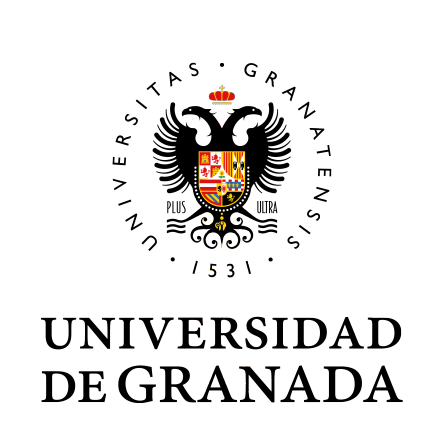
\includegraphics[scale=0.5]{img/ugr.png}\\

\textsc{\Large \asignatura{}\\[0.2cm]}
\textsc{GRADO EN INGENIERÍA INFORMÁTICA}\\[1cm]

\noindent\rule[-1ex]{\textwidth}{1pt}\\[1.5ex]
\textsc{{\Huge \titulo\\[0.5ex]}}
\textsc{{\Large \subtitulo\\}}
\noindent\rule[-1ex]{\textwidth}{2pt}\\[3.5ex]

\end{minipage}

\vspace{0.5cm}

\begin{minipage}{\textwidth}

\centering

\textbf{Autor}\\ {\autor{}}\\[2.5ex]
\textbf{Rama}\\ {Computación y Sistemas Inteligentes}\\[2.5ex]
\vspace{0.3cm}


\includegraphics[scale=0.3]{img/etsiit.jpeg}

\vspace{0.7cm}
\textsc{Escuela Técnica Superior de Ingenierías Informática y de Telecomunicación}\\
\vspace{1cm}
\textsc{Curso 2019-2020}
\end{minipage}
\end{titlepage}

\pagenumbering{arabic}
\tableofcontents
\thispagestyle{empty}				% No usar estilo en la pagina de indice

\newpage

\setlength{\parskip}{1em}


\section*{Ejercicio 1}
\addcontentsline{toc}{section}{Ejercicio 1}

\textbf{Identifique las semejanzas y diferencias entre los problemas de: a) clasificación de imágenes; b) detección de objetos;
c) segmentación de imágenes; d) segmentación de instancias.}

La \textbf{clasificación de imágenes} y consiste en, dada una imágen, catalogarla dependiendo del contenido de ésta. Por ejemplo, en la siguiente
imágen podemos clasificarla perfectamente como 'cat':
\begin{figure}[H]
\centering
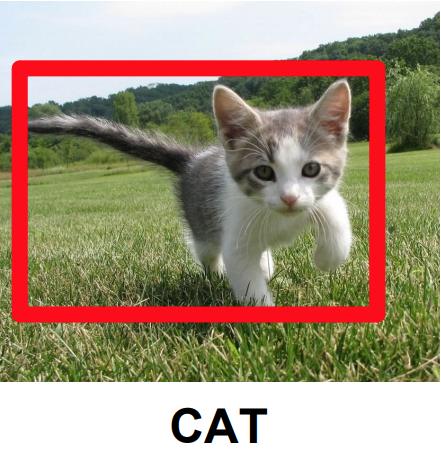
\includegraphics[scale=0.5]{img/classifier.png}
\caption{Clasificación de imágenes + localización}
\end{figure}

Por otra parte, la \textbf{detección de objetos} se parece a la clasificación en que el objetivo principal es el mismo, dependiendo de lo que aparezca en la
imagen, decir qué está reflejado en ella.

Lo que diferencia a la detección de objetos es que encuentra todos los objetos de una imagen, dibujando un cuadro delimitador alrededor de ellos.

En la imágen anterior, hemos visto que se dibuja un rectángulo, ya que ha detectado sólo un gato. Sin embargo, esto es lo que hace la detección de objetos cuando
hay más cosas en la escena:
\begin{figure}[H]
\centering
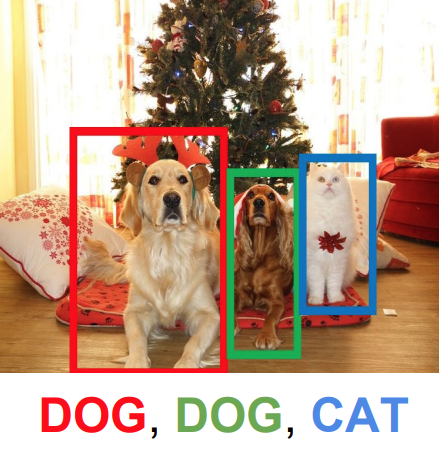
\includegraphics[scale=0.5]{img/object_detection.png}
\caption{Detección de objetos}
\end{figure}

Algo parecido ocurre con la segmentación de imágenes y la segmentación de instancias. Ambas consisten en, dada una imagen, clasificar cada píxel como perteneciente
a una clase en concreto. Si tomamos de ejemplo la misma imagen del gato, sería algo así:
\begin{figure}[H]
\centering
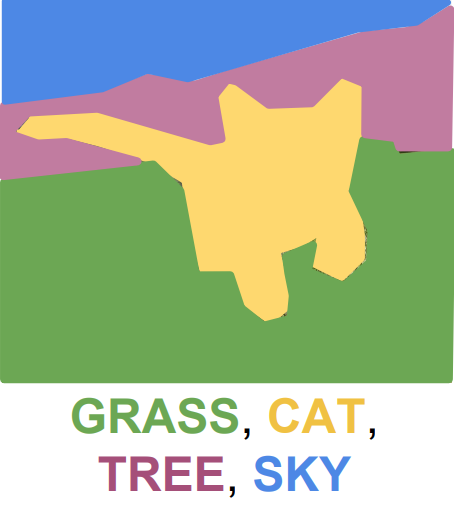
\includegraphics[scale=0.5]{img/semantic_segmentation.png}
\caption{Segmentación de imágenes}
\end{figure}

No obstante, lo que las diferencia la una de la otra es que, la \textbf{segmentación de imágenes} no crea máscaras para cada objeto individual en la escena. Por
ejemplo, si tuviesemos más de una gato en la foto anterior, nos lo fusionaría y detectaría todo como 'cat'.

Esto con la \textbf{segmentación de instancias} no ocurre, ya que separa todos los objetos de una imagen y los clasifica como clases distintas (al igual que ocurría
con la detección de objetos). Veamos un ejemplo con la imagen anterior:
\begin{figure}[H]
\centering
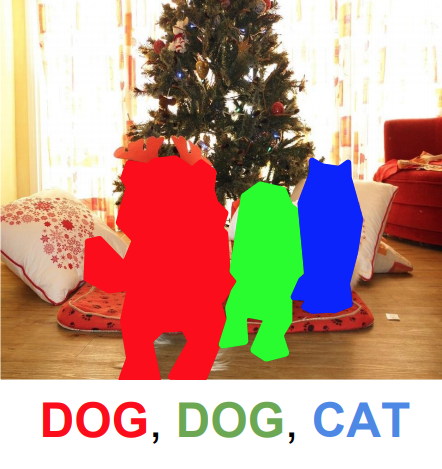
\includegraphics[scale=0.5]{img/image_segmentation.png}
\caption{Segmentación de instancias}
\end{figure}


\section*{Ejercicio 2}
\addcontentsline{toc}{section}{Ejercicio 2}

\textbf{¿Cuál es la técnica de búsqueda estándar para la detección de objetos en una imagen? Identifique pros y contras de la misma e indique
posibles soluciones para estos últimos.}

Esta técnica se la conoce como \textbf{\textit{Sliding Window Detection}}, el cual es un algoritmo capaz de detectar objetos en varios pasos bastante simples y que
realiza una búsqueda exhaustiva sobre la posición y la escala (puede usar una ventana del mismo tamaño sobre una pirámide espacial de imágenes).

Las desventajas que tiene son las siguientes:
\begin{itemize}
	\item \textit{Objetos de distintos tamaños}. Los objetos pueden aparecer con tamaños distintos en la imagen. Para solucionar esto se ha propuesto analizar
          la imagen a múltiples escalas con un tamaño de ventana prefijado. Altenativamente, también podemos analizar la imagen con distintos tamaños y proporciones
          de ventana.
	\item \textit{Variada relación de aspecto}. La ventana necesaria para analizar, por ejemplo, un gato de frente que un gato de perfil, no será la misma.
		  Es difícil encontrar una solución concreta para este problema, pero se podría ajustar la ventana a lo que estamos intentando hallar (para un semáforo,
          no elegir una ventana cuadrada, sería más bien alargada).
	\item \textit{Superposición de objetos y múltiples respuestas}. Dos o más ventanas pueden reconocer el mismo objeto, no obstante, cada una de estas múltiples
		  respuestas tienen distintos pesos. Tendremos que realizar una supresión de no máximos (también para las distintas escalas) y quedarnos con el mejor.
\end{itemize}


\section*{Ejercicio 3}
\addcontentsline{toc}{section}{Ejercicio 3}

\textbf{Considere la aproximación que extrae una serie de características en cada píxel de la imagen para decidir si hay contorno o no. Diga si existe algún
paralelismo entre la forma de actuar de esta técnica y el algoritmo de Canny. En caso positivo identifique cuales son los elementos comunes y en que se
diferencian los distintos.}

Una aproximación que hace esto es la \textbf{\textit{Selective Search}}, la cual no tiene aspectos muy similares al algoritmo de $Canny$. La búsqueda selectiva
extrae una serie de características para cada píxel y realiza una agrupación jerárquica basándose en similitudes entre texturas, tamaños, forma y color; mientras
que $Canny$ simplemente realiza una detección de contornos mediante histéresis. En caso de utilizar la búsqueda selectiva para detección de contornos, se podrían
obtener diferenciando entre unos segmentos detectados y otros.

Como similitud podemos comentar que ambos tienen en cuenta las distintas escalas de a imagen, con la diferencia de que la búsqueda selectiva utiliza un algoritmo
jerárquico, y $Canny$ detecta los contornos de escalas más grandes (sin fijarse tanto en los detalles) aumentando un valor de $\sigma$ y viceversa. También hacen
uso de la derivada de la Gaussiana para hacer un filtrado de la imagen.


\section*{Ejercicio 4}
\addcontentsline{toc}{section}{Ejercicio 4}

\textbf{Tanto el descriptor de SIFT como HOG usan el mismo tipo de información de la imagen pero en contextos distintos. Diga en que se parecen y en que son
distintos estos descriptores. Explique para que es útil cada uno de ellos.}

Ambos están basados en los gradientes de primer orden de la imagen, pero como su propio nombre indica, HoG simplemente realiza un histograma de los gradientes
agrupándolos segun su orientación; mientras que SIFT, después de hacer este histograma, realiza una interpolación entre ángulos vecinos y pondera los valores
de todo el descriptor mediante la Gaussiana.

Debido a esta ponderación Gaussiana que tiene SIFT, veo más útil utilizarlo para describir la importancia en un único punto; y HoG es más adecuado usarlo en
la clasificación de imágenes en general, ya que no tiene ese sesgo.


\section*{Ejercicio 5}
\addcontentsline{toc}{section}{Ejercicio 5}

\textbf{Observando el funcionamiento global de una CNN, identifique que dos procesos fundamentales definen lo que se realiza en un pase hacia delante de una
imagen por la red. Asocie las capas que conozca a cada uno de ellos.}

\begin{enumerate}
    \item Utilizar capas convolucionales con su activación 'ReLU', 'linear', 'tanh'..., capas de $pooling$ o algunas funciones de regularización como
          \textit{Dropout} o \textit{BatchNormalization}.
    \item Utilizar un clasificador con capas totalmente conectadas para realizar la predicción. También contarán con su función de activación (siendo la
          última 'softmax' para obtener las probabilidades de cada clase como salida).
\end{enumerate}



\section*{Ejercicio 6}
\addcontentsline{toc}{section}{Ejercicio 6}

\textbf{Se ha visto que el aumento de la profundidad de una CNN es un factor muy relevante para la extracción de características en problemas complejos, sin
embargo este enfoque añade nuevos problemas. Identifique cuales son y qué soluciones conoce para superarlos.}

Aumentar la profundida en una red neuronal de forma excesiva nos puede llevar al \textbf{sobreaprendizaje}, ya que la función de salida obtenida se ajusta casi por
completo al conjunto de entrenamiento. Una solución que podemos aplicar es el aumento del conjunto de datos (técnicas como \textit{horizontal flip}, o hacer zoom en
partes de la imagen son un ejemplo de esto). Otra solución para evitar el sobreaprendizaje es regularizar los datos introduciendo capas como \textit{Dropout} o
\textit{BatchNormalization}.

Por otra parte, al hacer \textbf{\textit{backpropagation}} se pierde precisión y los gradientes también van disminuyendo. Este problema es más difícil de solucionar,
ya que tendríamos que buscar nuevos métodos, como puede ser la ejecución capa por capa o utilizar clasificadores auxiliares en distintos niveles de la red neuronal
(como hace GoogleNet).


\section*{Ejercicio 7}
\addcontentsline{toc}{section}{Ejercicio 7}

\textbf{Existe actualmente alternativas de interés al aumento de la profundidad para el diseño de CNN. En caso afirmativo diga cuál/es y como son.}

La primera alternativa sería el \textbf{desacoplamiento de nodos}, que elimina la conexión entre el nodo de la capa actual y el de la siguiente, ya sea poniéndolo
a 0 con $Dropout$ o con $BatchNormalization$.

Otra posible alternativa sería la que utiliza $DenseNet$, que aumenta el número de conexiones entre una capas conectando la actual con todas las anteriores a ella
(aumento de \textbf{densidad}).

También tenemos el uso de múltiples escalas simultáneamente, es decir, aumentar la \textbf{anchura} de una red para así poder extraer más características.



\section*{Ejercicio 8}
\addcontentsline{toc}{section}{Ejercicio 8}

\textbf{Considere una aproximación clásica al reconocimiento de escenas en donde extraemos de la imagen un vector de características y lo usamos para decidir la
clase de cada imagen. Compare este procedimiento con el uso de una CNN para el mismo problema. ¿Hay conexión entre ambas aproximaciones? En caso afirmativo indique
en que parecen y en que son distintas.}

La arquitectura y los pasos que seguimos en una aproximación clásica son exactamente los mismos que los que utilizamos en la actualidad, primero se hacía la
extracción de características y luego se aprendía un clasificador.

La diferencia es que en la aproximación clásica, la extracción de características las tenía que hacer la persona manualmente y lo único que se aprendía era el
clasificador; mientras que en las CNN actuales aprendemos tanto el clasificador como las características.


\section*{Ejercicio 9}
\addcontentsline{toc}{section}{Ejercicio 9}

\textbf{¿Cómo evoluciona el campo receptivo de las neuronas de una CNN con la profundidad de la capas? ¿Se solapan los campos receptivos de las distintas neuronas de
una misma profundidad? ¿Es este hecho algo positivo o negativo de cara a un mejor funcionamiento?}

El campo receptivo es una región local en el volumen de salida de la capa anterior a la que está conectada una neurona. Si tenemos en cuenta que esta región es un tensor
3D con una profundidad igual a la profundidad del volumen en la capa anterior, podemos decir que cuanto más profunda sea nuestra red, \textbf{más se va a incrementar el
campo receptivo}. El submuestreo, por ejemplo, aumentaría el tamaño del campo receptivo multiplicativamente.

El \textbf{área superpuesta} depende del tamaño del \textit{'kernel'} y del \textit{'stride'}, ya que el \textit{stride} desplazaría el kernel en la capa siguiente.
Los \textit{strides} más grandes darían lugar a una menor superposición, mientras que los \textit{kernels} más grandes darían lugar a una mayor superposición. No hay
superposición solo si el \textit{stride} es igual al tamaño del \textit{kernel}.

La superposición lo que hace es aprovechar la fuerte coherencia espacial que suelen tener las imágenes, es decir, nos ayuda a cubrir todo el campo visual. No obstante,
una superposición excesiva puede hacer que perdamos demasiada información de lo que tenemos 'en primer plano' por así decirlo.


\section*{Ejercicio 10}
\addcontentsline{toc}{section}{Ejercicio 10}

\textbf{¿Qué operación es central en el proceso de aprendizaje y optmización de una CNN?}




\section*{Ejercicio 11}
\addcontentsline{toc}{section}{Ejercicio 11}

\textbf{Compare los modelos de detección de objetos basados en aproximaciones clásicas y los basados en CNN y diga que dos procesos comunes a ambas aproximaciones han
sido muy mejorados en los modelos CNN. Indique cómo.}

El enfoque tradicional realiza la \textbf{detección de objetos} mediante técnicas bien establecidas como SIFT, SURF, BRIEF, etc; y posteriormente se extraen las
características para hacer la \textbf{clasificación de imágenes}. Si un número significativo de características de una bolsa de palabras está en otra imagen, la imagen
se clasifica como un objeto en específico.

La dificultad con este enfoque tradicional es que es necesario elegir qué características son importantes en cada imagen dada, y a medida que aumenta el número de clases
se vuelve más complicado (es el criterio ingeniero el que decide qué características describen mejor los objetos).

Los \textbf{modelos CNN} introdujeron el concepto \textit{end-to-end}, donde solo se recibe un conjunto de datos con todas sus clases y se entrena sobre ellos. Las redes
neuronales descubren patrones en las imágenes (ya sea detección de bordes, de esquinas...) y automáticamente extrae las características más descriptivas con respecto a
cada clase.


\section*{Ejercicio 12}
\addcontentsline{toc}{section}{Ejercicio 12}

\textbf{Es posible construir arquitecturas CNN que sean independientes de las dimensiones de la imagen de entrada. En caso afirmativo diga cómo hacerlo y cómo
interpretar la salida.}

La primera idea que se nos viene a la cabeza sería el preprocesamiento de los datos, ya sea cambiando el tamaño de las imágenes, recortándolas o realizando cualquier
transformación. Sin embargo, quitando la pérdida de información producida, creo que no es lo que se pide exactamente en el ejercicio.

Lo que se pide es buscar una arquitectura CNN que reciba cualquier tipo de imagen sin preprocesar. Para este caso tenemos varias soluciones:
\begin{itemize}
	\item \textbf{Fully Convolutional Networks (FCN)}. No tienen limitaciones en el tamaño de entrada porque una vez que se describe el tamaño del $kernel$ y los canales,
		  la convolución produce una salida con las dimensiones correspondientes a la entrada (posiblemente muestreadas) para cada capa.
	\item \textbf{\textit{Pooling}}. Podríamos aplicar alguna técnica de \textit{pooling} al final de una capa convolucional que vaya a una capa FC (Fully Connected). De
		  esta forma podemos transformar el tensor de salida de dimensiones $(N, H, W, C)$ a un tensor de dimensiones $(N, 1, 1, C)$, donde la N es el número de muestras
		  elegido, H y W son altura y anchura, y la C es el número de canales del tensor.
	\item \textbf{\textit{ROI Pooling}}. Esta técnica también es una técnica de $pooling$, pero lo que la diferencia de las anteriores, es que la agrupación la adaptamos
		  a las regiones de interés. Podemos pasar la imagen completa a la CNN ya que podemos utilizar el mismo mapa de características para todas las propuestas y además
		  el número de canales de entrada es el mismo que el de salida para cada una de ellas.


\end{itemize}


\section*{Ejercicio 13}
\addcontentsline{toc}{section}{Ejercicio 13}

\textbf{Suponga que entrenamos una arquitectura Lenet-5 para clasificar imágenes 128x128 de 5 clases distintas. Diga que cambios deberían de hacerse en la arquitectura
del modelo para que se capaz de detectar las zonas de la imagen donde aparecen alguno de los objetos con los que fue entrenada.}



\section*{Ejercicio 14}
\addcontentsline{toc}{section}{Ejercicio 14}

\textbf{Argumente por qué la transformación de un tensor de dimensiones 128x32x32 en otro de dimensiones 256x16x16, usando una convolución 3x3 con stride=2, tiene sentido
que pueda ser aproximada por una secuencia de tres convoluciones: convolución 1x1 + convolución 3x3 + convolución 1x1. Diga también qué papel juegan cada una de las tres
convoluciones.}

Al decir 'tiene sentido' no se si la pregunta va referida a si se puede realizar el cálculo haciéndolo más eficiente, o a que el resultado obtenido será similar al que
obtendríamos con la convolución 3x3, asi que voy a analizar los dos puntos de vista.

\textbf{¿Por qué es más eficiente?} Si utilizamos 3 convoluciones en vez de 1 podremos reducir la profundidad de los tensores generados, y por tanto, se reducen también
la cantidad de operaciones realizadas.
\begin{equation}
	n\_operaciones = prof_{ini} * kernel * prof_{obj} * alt_{obj} * anc_{obj}
\end{equation}

Utilizando una única convolución 3x3 al tensor de 128x32x32 nos da el siguiente resultado:
\begin{equation}
	n\_operaciones = 128 * (3*3) * 256 * 16 * 16 = 75.497.472
\end{equation}

Por otro lado, vamos a realizar las operaciones para llegar al tensor de salida utilizando las 3 convoluciones, calculando los dos tensores intermedios y sumando los
resultados obtenidos:
\begin{eqnarray*}
	n\_operaciones & = & (128 * (1*1) * 64 * 32 * 32) + \\
	& & (64 * (3*3) * 64 * 16 * 16) + \\
	& & (64 * (1*1) * 256 * 16 * 16) = 22.020.096 \\
\end{eqnarray*}

Como podemos ver, la cantidad de operaciones se ha reducido considerablemente. Esto se debe a que hemos reducido a la mitad la profundidad en las dos primeras convoluciones,
así reducir la dimensión a 16x16 de una forma más eficiente, y posteriormente aumentar a la profundidad de 256 objetivo.

\textbf{¿Por qué el cálculo no es diferente?} Podríamos realizarlo de esta manera ya que la capa de convolución 1x1 actúa como una capa totalmente conectada en cuanto a píxeles,
es decir, no cambiamos nada a nivel espacial (el alto y el ancho siguen siendo el mismo), pero reducimos el número de canales obteniendo los valores más significativos.

Si la red está bien entrenada, sería capaz de representar la información más representativa con menos características.


\section*{Ejercicio 15}
\addcontentsline{toc}{section}{Ejercicio 15}

\textbf{Identifique una propiedad técnica de los modelos CNN que permite pensar que podrían llegar a aproximar con precisión las características del modelo de visión
humano, y que sin ella eso no sería posible. Explique bien su argumento.}

En los humanos, cuando observamos una imagen, la información pasa a través de cada cortex visual \textbf{como si fueran capas de la red}. Cada uno de ellos extrae un tipo
de información relevante, como pueden ser la ubicación espacial, color, tamaño, forma, etc.

La arquitectura de modelos CNN tienen la propiedad de activar las neuronas cuando este tipo de patrones o información relevante la encontramos en los píxeles de una imagen.
A su vez, se transmite entre capa y capa (cortex y cortex en el caso del cerebro).

Al igual que ocurre en las redes convoluciones, en nuestro cerebro no se van activando todas las neuronas linealmente, si no que algunas pueden permanecer inactivas y activarse
en otra fase del aprendizaje. Un ejemplo muy representativo de esto serían las capas de $Dropout$, aunque también existen otros métodos que reactivan neuronas inactivas.



\end{document}